\documentclass[unicode,aspectratio=169,12pt]{beamer}
\usepackage{luatexja}
\usepackage{graphicx}
\usepackage{booktabs}
\usepackage{array}
\usepackage{xcolor}
\usepackage{tikz}
\usetikzlibrary{arrows.meta,positioning,fit,shapes.geometric}

\usetheme{Madrid}
\usecolortheme{default}
\setbeamertemplate{navigation symbols}{}
\setbeamertemplate{footline}[frame number]
\graphicspath{{figures/}}

\definecolor{mainblue}{HTML}{2F6FBB}
\definecolor{safegreen}{HTML}{3F9B6D}
\definecolor{warnorange}{HTML}{E2A72E}
\definecolor{harmred}{HTML}{C94C4C}
\definecolor{softgray}{HTML}{F2F4F7}

\newcommand{\pp}{\mathrm{pp}}
\newcommand{\hsc}{HSC@0.5pp}
\newcommand{\source}{\texttt{source\_only}}
\newcommand{\replay}{\texttt{replay\_safe\_uniform}}

\title[EEG-MI OTTA]{EEG-MI cross-session OTTA における安全な適応方針の検討}
\subtitle{Replay-SafeCommit と非破壊な予測補正の検討}
\author{史研究室 M2 \quad 生川 聖也}
\date{2026年度 前期定期ゼミ}

\begin{document}

\begin{frame}
  \titlepage
\end{frame}

\begin{frame}{20分発表の流れ}
  \small
  \begin{enumerate}
    \item 背景・目的: EEG-MI と cross-session drift
    \item ベースモデル: TCFormer
    \item 問題: OTTA は誤更新で壊れる
    \item 評価軸: 平均精度だけでなく harm を見る
    \item 提案: Replay-SafeCommit
    \item 主結果: 安全制約下で +0.69pp, HSC=0/9
    \item 次の問い: 安全性だけでなく補正力を上げたい
    \item 補正力向上の検証1: 9被験者評価
    \item 補正力向上の検証2: seed 安定性評価
    \item 診断: model-state commit 回数は改善を説明しない
    \item 解釈: L1/L2 の非破壊補正が主因
    \item 今後: Commitless Memory-Corrected OTTA
    \item まとめ
  \end{enumerate}
  \vspace{0.8em}
  \begin{block}{今日の結論}
    本研究では、Replay-SafeCommit により subject-level harm を抑えた OTTA を実現する。
    さらに補正力を高める検証から、model-state commit よりも、非破壊な予測補正と external memory が重要であることが示唆された。
  \end{block}
\end{frame}

\section{背景}

\begin{frame}{背景: Active BCI と EEG-MI}
  \begin{columns}[T,onlytextwidth]
    \begin{column}{0.56\textwidth}
      \begin{itemize}
        \item BCI は脳活動からユーザーの意図を推定し、外部機器を操作する技術。
        \item 本研究は、ユーザーが能動的に運動を想起する \alert{Active BCI} を対象とする。
        \item EEG-MI では、左手・右手・足・舌などの運動想起を EEG から分類する。
        \item ゲーム応用では、事前キャリブレーションを増やさず、オンラインで安定に動くことが重要。
      \end{itemize}
    \end{column}
    \begin{column}{0.40\textwidth}
      \centering
      \begin{tikzpicture}[node distance=0.85cm,>=Latex,every node/.style={font=\small}]
        \node[draw,rounded corners,fill=softgray,minimum width=3.4cm,minimum height=0.75cm] (cue) {運動想起};
        \node[draw,rounded corners,fill=softgray,below=of cue,minimum width=3.4cm,minimum height=0.75cm] (eeg) {EEG 22ch};
        \node[draw,rounded corners,fill=mainblue!12,below=of eeg,minimum width=3.4cm,minimum height=0.75cm] (model) {分類モデル};
        \node[draw,rounded corners,fill=safegreen!18,below=of model,minimum width=3.4cm,minimum height=0.75cm] (control) {ゲーム操作};
        \draw[->,thick] (cue) -- (eeg);
        \draw[->,thick] (eeg) -- (model);
        \draw[->,thick] (model) -- (control);
      \end{tikzpicture}
    \end{column}
  \end{columns}
  \vspace{0.7em}
  \begin{block}{本研究の関心}
    学習済み EEG-MI 分類器を、session が変わっても安全に使い続けたい。
  \end{block}
\end{frame}

\begin{frame}{背景: EEG-MI では session 間の分布ずれが大きい}
  \begin{columns}[T,onlytextwidth]
    \begin{column}{0.56\textwidth}
      \begin{itemize}
        \item EEG-MI は、脳波から運動想起クラスを分類する Active BCI タスク。
        \item 同じ被験者でも、日・session・疲労・電極状態で特徴分布が変化する。
        \item 学習 session の分類器を評価 session にそのまま使うと、性能が落ちやすい。
      \end{itemize}
      \vspace{0.8em}
      \begin{block}{実用上の要求}
        再キャリブレーションを大きく増やさず、target session に逐次追従したい。
      \end{block}
    \end{column}
    \begin{column}{0.40\textwidth}
      \centering
      \begin{tikzpicture}[node distance=1.1cm,>=Latex]
        \node[draw,rounded corners,fill=softgray,minimum width=3.3cm,minimum height=0.8cm] (train) {session T で学習};
        \node[draw,rounded corners,fill=softgray,below=of train,minimum width=3.3cm,minimum height=0.8cm] (test) {session E で評価};
        \node[draw,rounded corners,fill=harmred!15,below=of test,minimum width=3.3cm,minimum height=0.8cm] (drop) {精度低下};
        \draw[->,thick] (train) -- node[right]{drift} (test);
        \draw[->,thick] (test) -- (drop);
      \end{tikzpicture}
    \end{column}
  \end{columns}
\end{frame}

\section{TCFormer}

\begin{frame}{ベースモデル: TCFormer}
  \begin{columns}[T,onlytextwidth]
    \begin{column}{0.46\textwidth}
      \begin{itemize}
        \item TCFormer は EEG-MI 向けの CNN + Transformer + TCN 型モデル。
        \item MK-CNN で空間・周波数特徴を抽出する。
        \item Transformer Encoder で大域的な依存関係を扱う。
        \item TCN で時間方向の文脈を分類に使う。
      \end{itemize}
    \end{column}
    \begin{column}{0.50\textwidth}
      \centering
      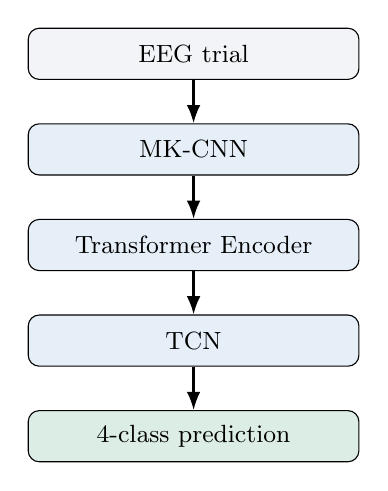
\begin{tikzpicture}[node distance=0.55cm,>=Latex,every node/.style={font=\small}]
        \node[draw,rounded corners,fill=softgray,minimum width=4.2cm,minimum height=0.65cm] (x) {EEG trial};
        \node[draw,rounded corners,fill=mainblue!12,below=of x,minimum width=4.2cm,minimum height=0.65cm] (mk) {MK-CNN};
        \node[draw,rounded corners,fill=mainblue!12,below=of mk,minimum width=4.2cm,minimum height=0.65cm] (tr) {Transformer Encoder};
        \node[draw,rounded corners,fill=mainblue!12,below=of tr,minimum width=4.2cm,minimum height=0.65cm] (tcn) {TCN};
        \node[draw,rounded corners,fill=safegreen!18,below=of tcn,minimum width=4.2cm,minimum height=0.65cm] (y) {4-class prediction};
        \draw[->,thick] (x) -- (mk);
        \draw[->,thick] (mk) -- (tr);
        \draw[->,thick] (tr) -- (tcn);
        \draw[->,thick] (tcn) -- (y);
      \end{tikzpicture}
    \end{column}
  \end{columns}
  \vspace{0.6em}
  \begin{block}{本研究での役割と限界}
    TCFormer を強い source model として用いる。ただし静的モデルのままでは target session の drift に追従できないため、test-time path に安全な適応機構を追加する。
  \end{block}
\end{frame}

\begin{frame}{問題: OTTA は有望だが、誤更新で壊れる}
  \begin{columns}[T,onlytextwidth]
    \begin{column}{0.54\textwidth}
      \begin{itemize}
        \item OTTA は target session の unlabeled stream を使って逐次適応する。
        \item drift 追従の可能性がある一方、正解ラベルがない。
        \item EEG では高信頼予測が正解とは限らない。
        \item 誤った trial で model state を更新すると、以降の trial に悪影響が残る。
      \end{itemize}
    \end{column}
    \begin{column}{0.42\textwidth}
      \centering
      \begin{tikzpicture}[node distance=0.9cm,>=Latex]
        \node[draw,rounded corners,fill=softgray,minimum width=3.6cm] (p) {高pmaxだが誤分類};
        \node[draw,rounded corners,fill=warnorange!25,below=of p,minimum width=3.6cm] (u) {誤った更新};
        \node[draw,rounded corners,fill=harmred!20,below=of u,minimum width=3.6cm] (c) {model state 汚染};
        \node[draw,rounded corners,fill=harmred!20,below=of c,minimum width=3.6cm] (h) {後続 trial も悪化};
        \draw[->,thick] (p) -- (u);
        \draw[->,thick] (u) -- (c);
        \draw[->,thick] (c) -- (h);
      \end{tikzpicture}
    \end{column}
  \end{columns}
  \vspace{0.8em}
  \begin{alertblock}{中心課題}
    OTTA では「適応するか」だけでなく、「どの状態を、いつ、どれだけ更新するか」を安全に決める必要がある。
  \end{alertblock}
\end{frame}

\begin{frame}{評価軸: 平均精度だけでなく harm を見る}
  \begin{table}
    \centering
    \begin{tabular}{p{0.27\textwidth}p{0.38\textwidth}p{0.24\textwidth}}
      \toprule
      指標 & 意味 & 目的 \\
      \midrule
      mean accuracy & 全被験者平均の精度 & 全体性能を見る \\
      $\Delta$ vs source & 適応なし baseline からの改善幅 & OTTA の価値を見る \\
      worst $\Delta$ & 最も悪化した被験者の変化量 & worst-case harm を見る \\
      \hsc & 0.5pp 以上悪化した被験者数 & material harm を数える \\
      \bottomrule
    \end{tabular}
  \end{table}
  \vspace{0.5em}
  \begin{block}{目標}
    平均精度を上げるだけでなく、被験者単位で大きく壊さない OTTA を作る。
  \end{block}
\end{frame}

\section{Replay-SafeCommit}

\begin{frame}{提案: Replay-SafeCommit}
  \begin{block}{観察}
    forward-only OTTA では、current trial の即時 margin / SAL 比較だけでは commit の真の効果を測りにくい。
  \end{block}
  \vspace{0.5em}
  \begin{block}{提案}
    候補更新を仮適用し、過去の高信頼 trial を保持した replay buffer 上で simulated reward を測ってから commit する。
  \end{block}
  \vspace{0.5em}
  \[
    \mathrm{sim\_score}
    = w_{\mathrm{acc}}\Delta \mathrm{replay\_acc}
    + w_{\mathrm{margin}}\Delta \mathrm{replay\_margin}
    + w_{\mathrm{proto}}\Delta \mathrm{replay\_proto\_cos}
  \]
  \centering
  \large $\mathrm{sim\_score} > 0$ の候補だけ採用する。
\end{frame}

\begin{frame}{主結果: 安全制約下では Replay-SafeCommit が最も堅い}
  \begin{table}
    \centering
    \begin{tabular}{lrrrr}
      \toprule
      method & mean & $\Delta$ & worst $\Delta$ & \hsc \\
      \midrule
      \source & 82.72 & +0.00 & +0.00 & 0/9 \\
      \texttt{policy\_safe\_no\_shallow} & 83.14 & +0.42 & -0.35 & 0/9 \\
      \replay & \textbf{83.41} & \textbf{+0.69} & -0.35 & \textbf{0/9} \\
      \bottomrule
    \end{tabular}
  \end{table}
  \vspace{0.6em}
  \begin{block}{言えること}
    同一実験内の \source に対して、Replay-SafeCommit は平均精度を +0.69pp 改善し、0.5pp以上悪化した被験者を出さなかった。
  \end{block}
\end{frame}

\begin{frame}{次の問い: 安全性だけでなく補正力を上げたい}
  \begin{columns}[T,onlytextwidth]
    \begin{column}{0.48\textwidth}
      \begin{block}{提案手法で見えたこと}
        \begin{itemize}
          \item Replay-SafeCommit は安全
          \item ただし平均改善は +0.69pp
          \item 補正器そのものはまだ弱い
        \end{itemize}
      \end{block}
    \end{column}
    \begin{column}{0.48\textwidth}
      \begin{alertblock}{次の問い}
        \begin{itemize}
          \item model state をすぐ動かさずに補正できるか
          \item L1: prediction correction
          \item L2: external memory
          \item L3: model-state commit
        \end{itemize}
      \end{alertblock}
    \end{column}
  \end{columns}
  \vspace{0.5em}
  \small
  以降では、9被験者評価と、S2/S4/S6/S7 $\times$ 複数 seed の安定性評価で切り分ける。
\end{frame}

\begin{frame}{補正力向上の検証1: 9被験者では精度向上シグナルが出た}
  \begin{columns}[T,onlytextwidth]
    \begin{column}{0.63\textwidth}
      \includegraphics[width=\textwidth]{fig_plan_c_key_results.png}
    \end{column}
    \begin{column}{0.34\textwidth}
      \begin{itemize}
        \item best DC は 83.95\%, +1.23pp。
        \item \replay は 83.41\%, +0.69pp, HSC=0/9。
        \item best DC は S4 で -1.38pp 悪化し、HSC=1/9。
        \item 安全制約 HSC=0 では \replay が最も堅い。
      \end{itemize}
    \end{column}
  \end{columns}
\end{frame}

\begin{frame}{補正力向上の検証2: seed安定性では Replay-SafeCommit が優位}
  \begin{columns}[T,onlytextwidth]
    \begin{column}{0.63\textwidth}
      \includegraphics[width=\textwidth]{fig_plan_b_key_results.png}
    \end{column}
    \begin{column}{0.34\textwidth}
      \begin{itemize}
        \item best DC は 76.13\%, +0.49pp。
        \item ただし HSC=4/12。
        \item \replay は 76.01\%, +0.38pp, HSC=1/12。
        \item seed 安定性込みでは \replay がより安全側。
      \end{itemize}
    \end{column}
  \end{columns}
\end{frame}

\begin{frame}{診断: best gain は model-state commit では説明できない}
  \begin{figure}
    \centering
    \includegraphics[width=0.94\textwidth]{fig_l3_commit_diagnostics.png}
  \end{figure}
  \vspace{-0.5em}
  \begin{block}{読み取り}
    同じ精度なのに commit 回数が 0, 33, 111, 150 と変わる。さらに 9被験者評価で最も平均精度が高い variant は L3 commit が 0 回。
  \end{block}
\end{frame}

\section{解釈と方針}

\begin{frame}{解釈: L1/L2 の非破壊補正が主因}
  \begin{block}{Replay-SafeCommit の設計思想}
    replay evidence が溜まるまで model-state commit を遅延する階層型 OTTA policy。
  \end{block}
  \vspace{0.6em}
  \begin{alertblock}{補正力向上検証からの示唆}
    強いシグナルが出たのは L3 commit の遅延ではなく、\alert{model state を動かさない prediction correction と external memory} である。
  \end{alertblock}
  \vspace{0.6em}
  \begin{block}{新しい中心仮説}
    EEG-MI OTTA では、まず非破壊な memory-corrected prediction を行い、model-state commit は例外的に扱う方が、平均精度と harm 抑制の両立に有利である。
  \end{block}
\end{frame}

\begin{frame}{今後: Commitless Memory-Corrected OTTA}
  \begin{enumerate}
    \item \textbf{安全な基準}: Replay-SafeCommit を subject-level harm 抑制の基準にする。
    \item \textbf{新しい中核}: model state を動かさず、external memory で posterior を補正する。
    \item \textbf{改善対象}: correction strength と memory admission を中心に設計する。
    \item \textbf{失敗条件}: S4/S6 で memory reliability, class entropy, corrected-only rate を見る。
    \item \textbf{L3の扱い}: commit は補助仮説に下げ、controlled drift 条件で効くかを検証する。
  \end{enumerate}
  \vspace{0.5em}
  \begin{block}{新規性の置き方}
    強い更新候補を増やすのではなく、非破壊補正を第一選択にし、model-state commit を例外化する OTTA policy として整理する。
  \end{block}
\end{frame}

\begin{frame}{まとめ}
  \begin{itemize}
    \item Replay-SafeCommit は \source から +0.69pp、HSC=0/9 を達成した。
    \item 補正力向上の検証では、DC 系が 9被験者評価で最大 +1.23pp まで伸びた。
    \item しかし seed 安定性では DC 系の HSC が増え、Replay-SafeCommit の安全性が確認された。
    \item L3 commit の効果はまだ示せず、得られた gain は L1/L2、つまり非破壊補正と external memory が主因と考えるべき。
    \item 次は Commitless Memory-Corrected OTTA として、memory reliability と correction safety を詰める。
  \end{itemize}
\end{frame}

\appendix

\begin{frame}{Appendix: Safety--Gain tradeoff}
  \begin{figure}
    \centering
    \includegraphics[width=0.96\textwidth]{fig_safety_tradeoff.png}
  \end{figure}
  \vspace{-0.5em}
  \centering
  \small 右へ行くほど平均改善、上へ行くほど worst-case harm が小さい。理想は右上。
\end{frame}

\begin{frame}{Appendix: seed-stability subject--seed delta}
  \begin{figure}
    \centering
    \includegraphics[width=0.93\textwidth]{fig_plan_b_subject_seed_delta.png}
  \end{figure}
  \vspace{-0.4em}
  \begin{itemize}
    \item DC high mean は S2/S7 を大きく救う。
    \item 一方で S4/S6 の複数 seed で悪化しやすい。
  \end{itemize}
\end{frame}

\begin{frame}{Appendix: 仮説ごとの支持状況}
  \begin{columns}[T,onlytextwidth]
    \begin{column}{0.48\textwidth}
      \begin{block}{支持された}
        \begin{itemize}
          \item L1 prediction correction には精度向上シグナルがある。
          \item L2 external memory は target 分布の利用として有望。
          \item Replay-SafeCommit は安全な基準点として強い。
        \end{itemize}
      \end{block}
    \end{column}
    \begin{column}{0.48\textwidth}
      \begin{alertblock}{まだ支持されない}
        \begin{itemize}
          \item L3 replay-gated commit が性能改善の主因である。
          \item DC-Replay が seed 安定性込みで Replay-SafeCommit を超える。
          \item aggressive correction をそのまま採用して安全である。
        \end{itemize}
      \end{alertblock}
    \end{column}
  \end{columns}
\end{frame}

\begin{frame}{Appendix: 9-subject per-subject delta}
  \begin{figure}
    \centering
    \includegraphics[width=0.95\textwidth]{fig_plan_c_per_subject_delta.png}
  \end{figure}
\end{frame}

\begin{frame}{Appendix: 主要結果テーブル}
  \scriptsize
  \begin{table}
    \centering
    \begin{tabular}{llrrrr}
      \toprule
      eval & method & mean & $\Delta$ & worst $\Delta$ & \hsc \\
      \midrule
      9subj & \source & 82.72 & +0.00 & +0.00 & 0/9 \\
      9subj & \replay & 83.41 & +0.69 & -0.35 & 0/9 \\
      9subj & DC safe grid & 83.37 & +0.66 & -0.35 & 0/9 \\
      9subj & DC high mean & 83.95 & +1.23 & -1.38 & 1/9 \\
      \midrule
      seed & \source & 75.63 & +0.00 & +0.00 & 0/12 \\
      seed & \replay & 76.01 & +0.38 & -0.69 & 1/12 \\
      seed & DC L1+L2 & 75.90 & +0.26 & -1.04 & 3/12 \\
      seed & DC best & 76.13 & +0.49 & -1.04 & 4/12 \\
      \bottomrule
    \end{tabular}
  \end{table}
\end{frame}

\begin{frame}{Appendix: 参考文献}
  \small
  \begin{itemize}
    \item Altaheri et al., ``Temporal convolutional transformer for EEG based motor imagery decoding,'' Scientific Reports, 2025.
    \item Luo et al., ``Bayesian Test-Time Adaptation via Dirichlet Feature Projection and GMM-Driven Inference for Motor Imagery EEG Decoding,'' ICLR 2026.
    \item 第二回班ゼミ資料: Replay-SafeCommit と BTTA-DG 調査。
  \end{itemize}
\end{frame}

\end{document}
